% Auto-generated by eval_pipeline/bab4_artifact_export.py
% These figures assume this file is included from docs/proposal tugas akhir/Skripsi.tex.

\begin{figure}[htbp]
    \centering
    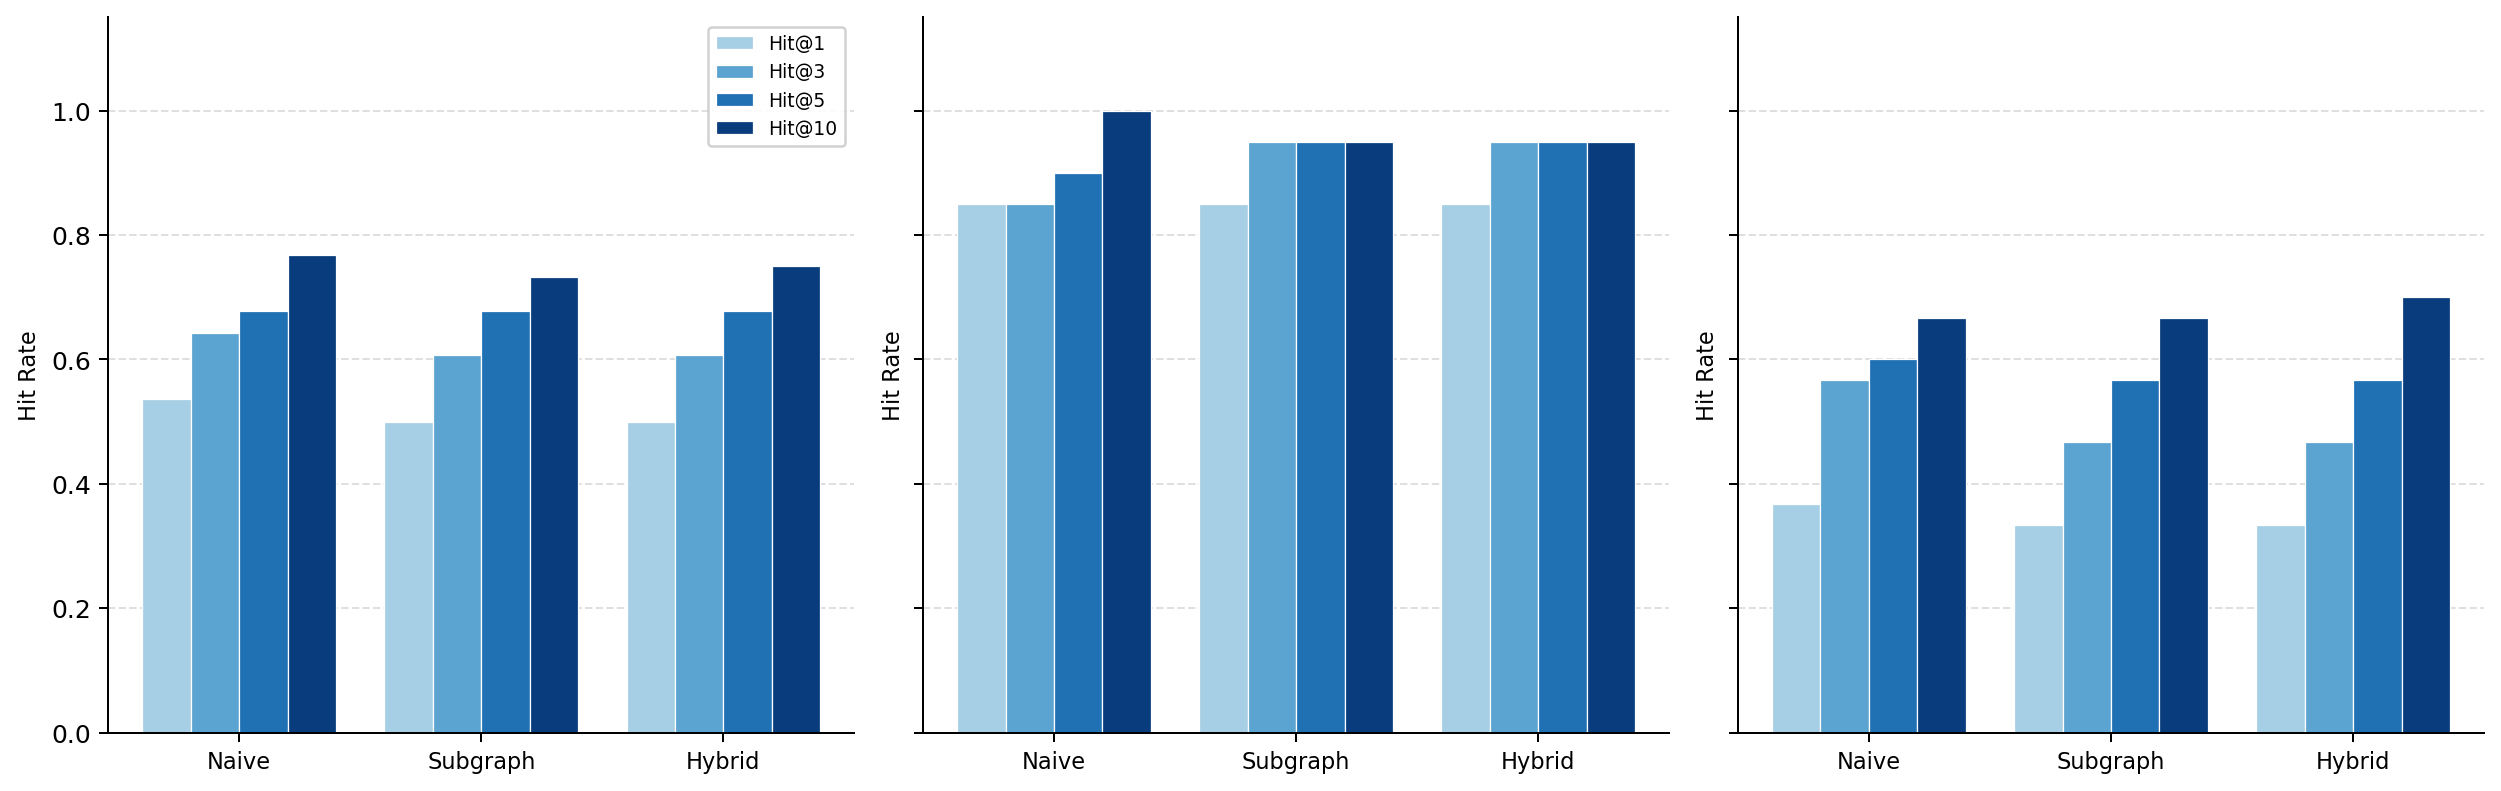
\includegraphics[width=0.82\linewidth]{Gambar/eval_layer1_hit_rate.png}
    \caption{Perbandingan Hit@K pada evaluasi retrieval.}
    \label{fig:eval-layer1-hit-rate}
\end{figure}

\begin{figure}[htbp]
    \centering
    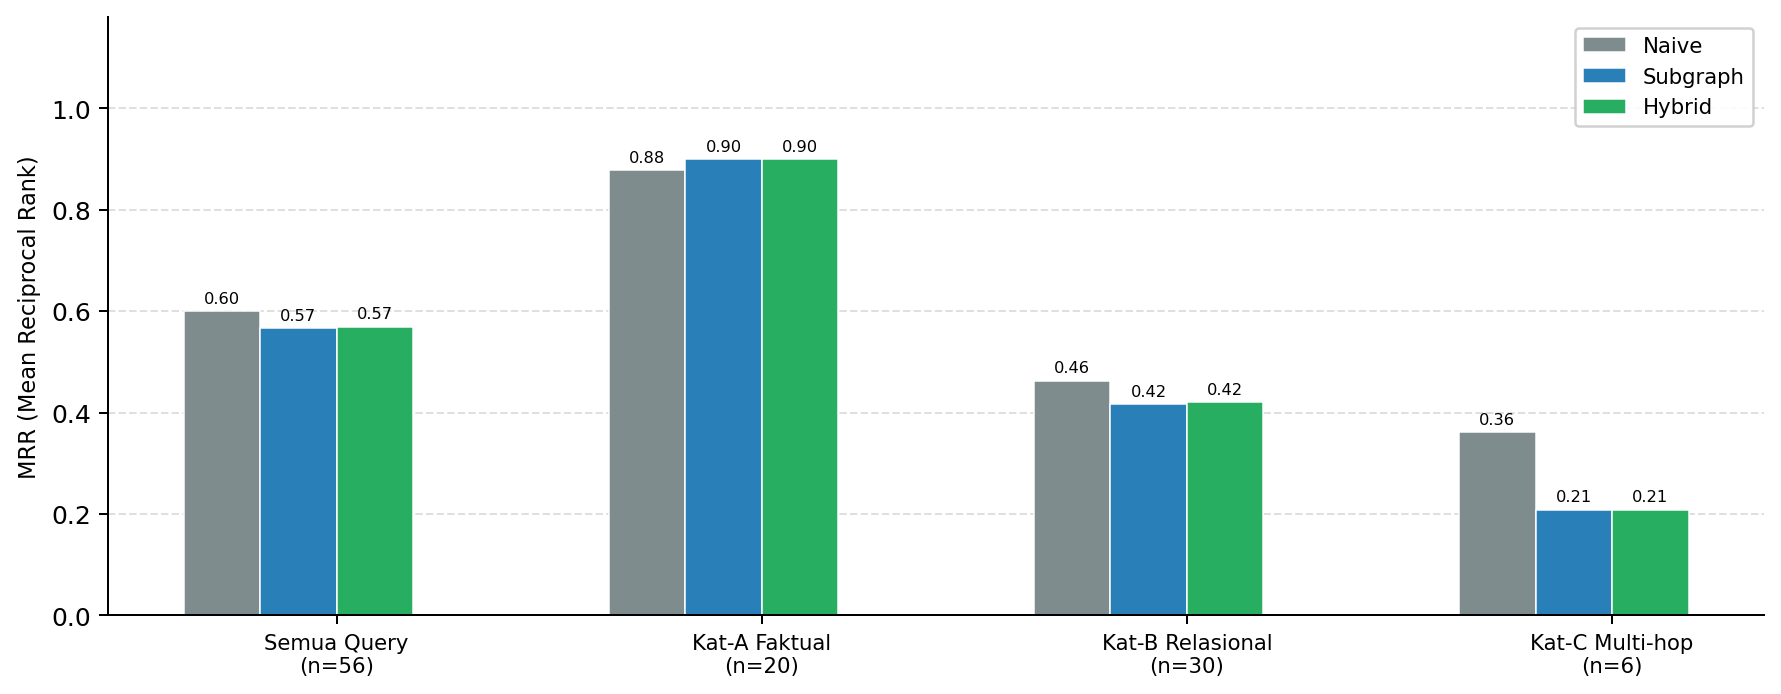
\includegraphics[width=0.82\linewidth]{Gambar/eval_layer1_mrr.png}
    \caption{Perbandingan Mean Reciprocal Rank pada evaluasi retrieval.}
    \label{fig:eval-layer1-mrr}
\end{figure}

\begin{figure}[htbp]
    \centering
    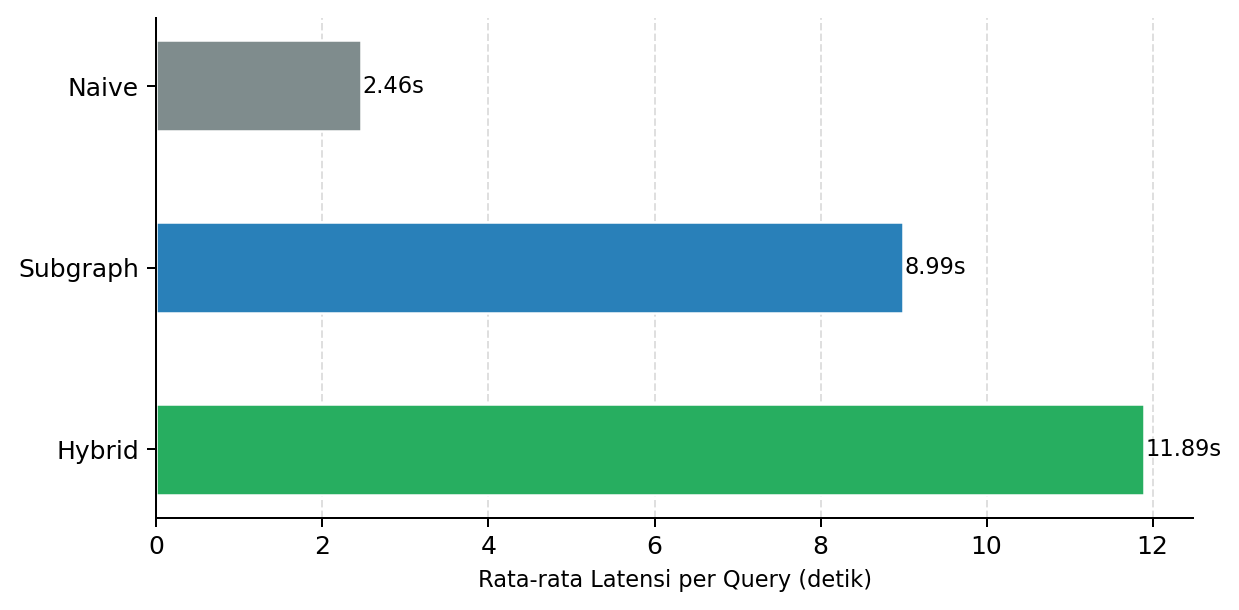
\includegraphics[width=0.78\linewidth]{Gambar/eval_layer1_latency.png}
    \caption{Rata-rata latensi retrieval pada setiap mode.}
    \label{fig:eval-layer1-latency}
\end{figure}

\begin{figure}[htbp]
    \centering
    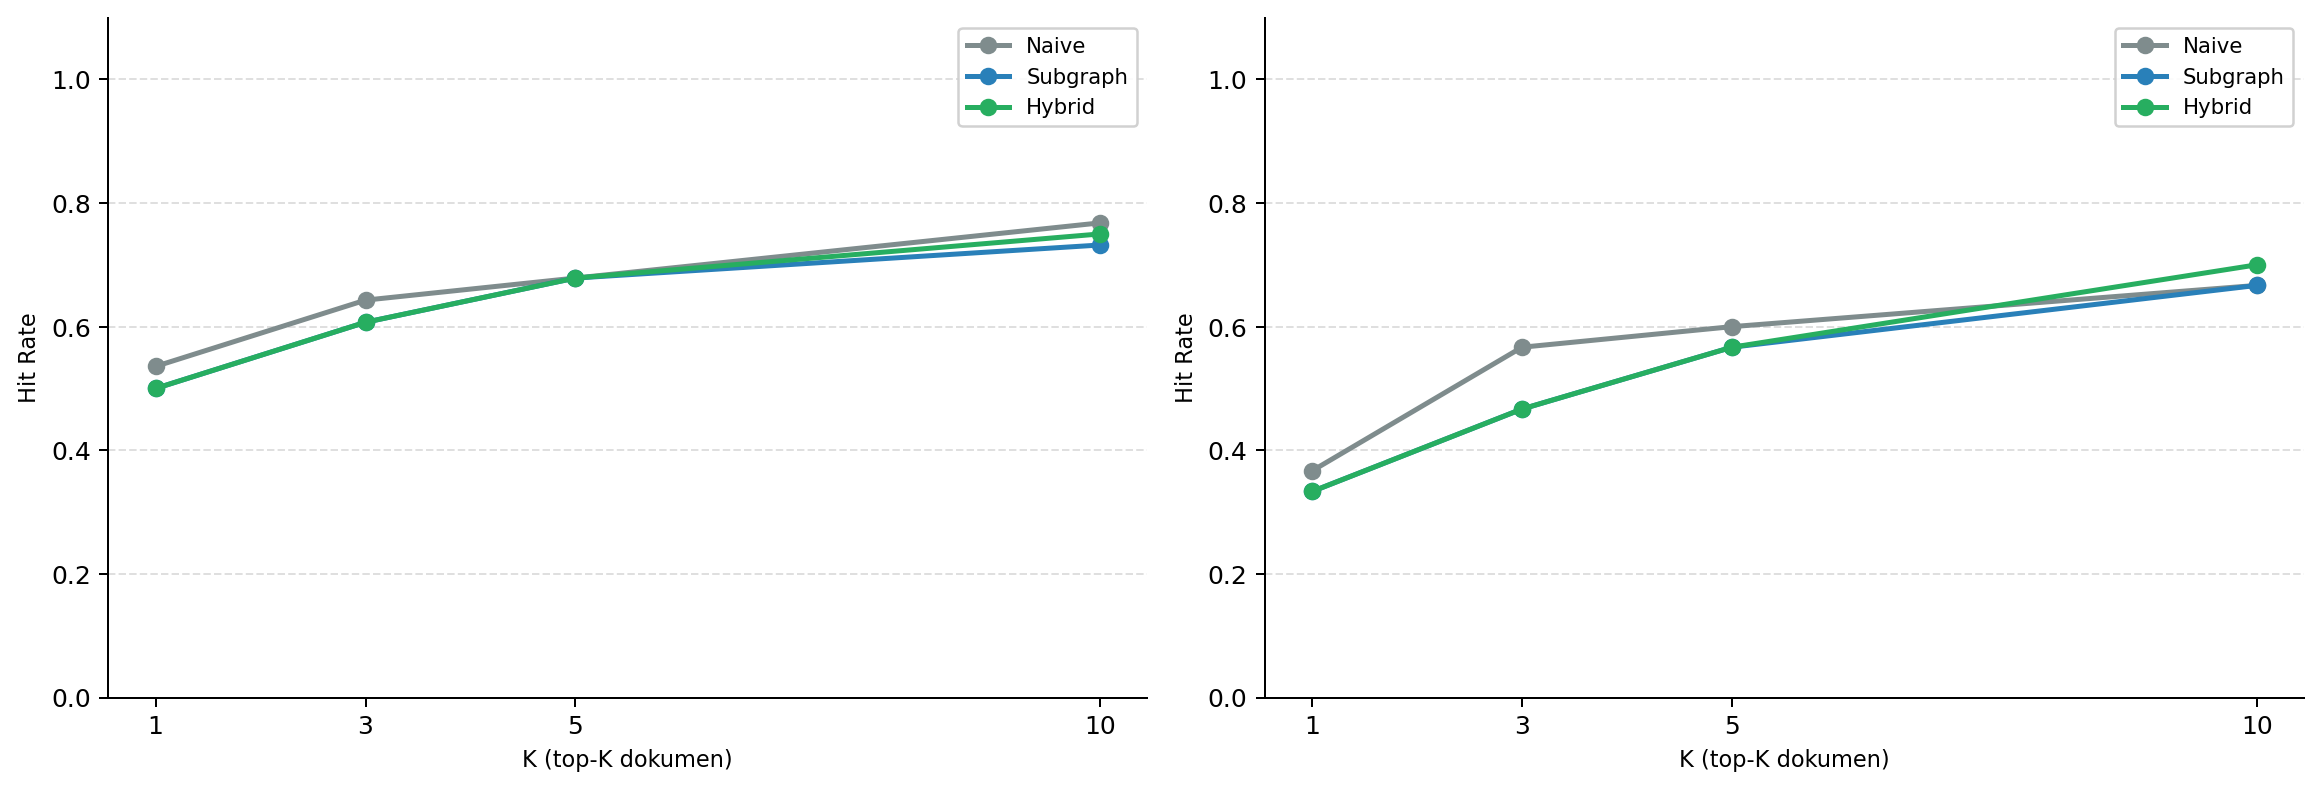
\includegraphics[width=0.86\linewidth]{Gambar/eval_layer3_hit_curves.png}
    \caption{Kurva Hit@K untuk membandingkan mode retrieval.}
    \label{fig:eval-layer3-hit-curves}
\end{figure}

\begin{figure}[htbp]
    \centering
    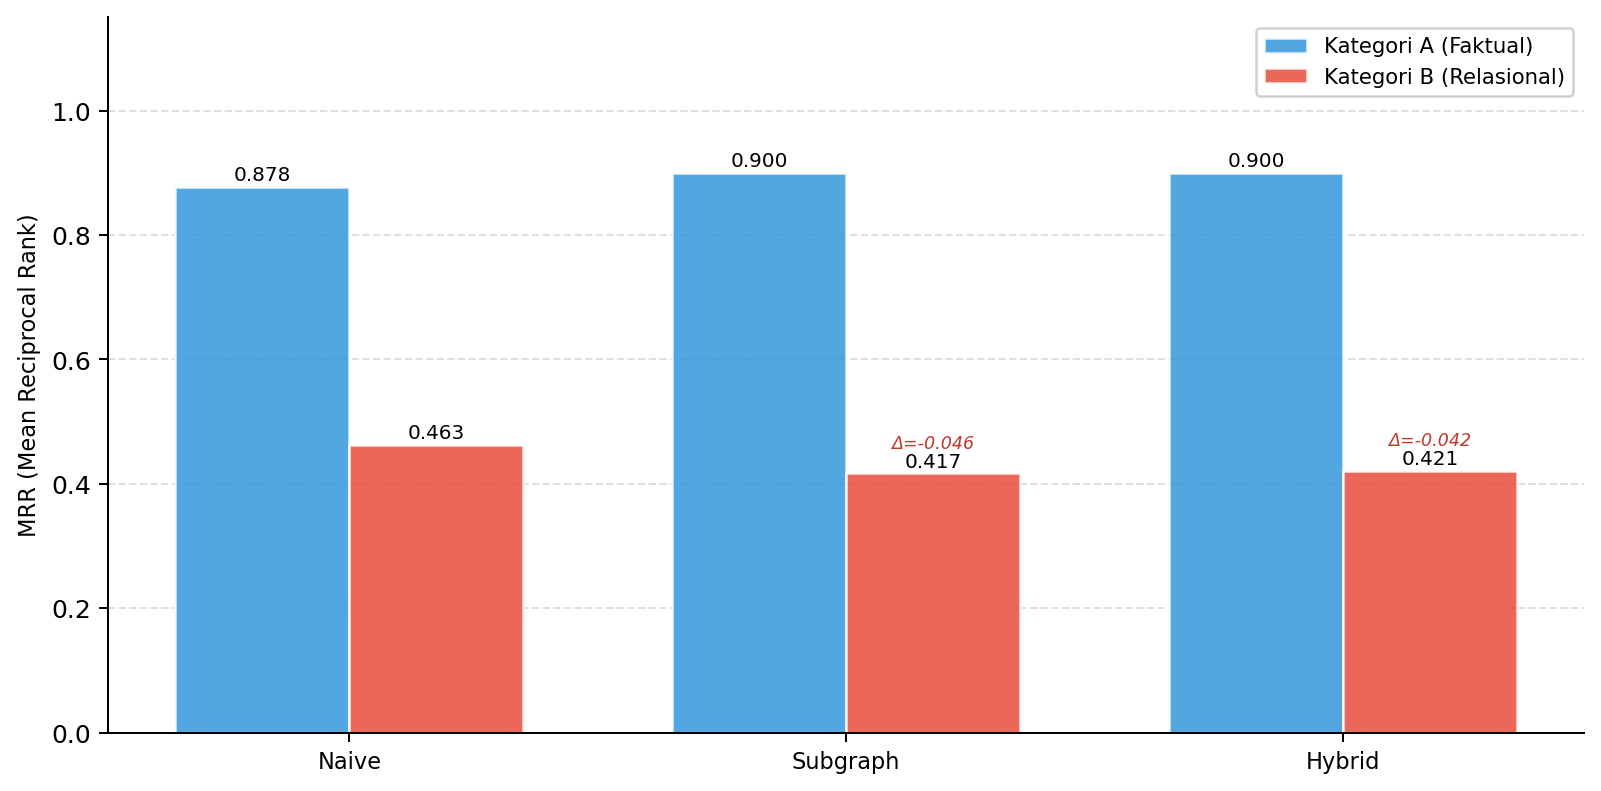
\includegraphics[width=0.86\linewidth]{Gambar/eval_layer3_mrr_by_category.png}
    \caption{MRR tiap mode retrieval berdasarkan kategori pertanyaan.}
    \label{fig:eval-layer3-mrr-category}
\end{figure}

\begin{figure}[htbp]
    \centering
    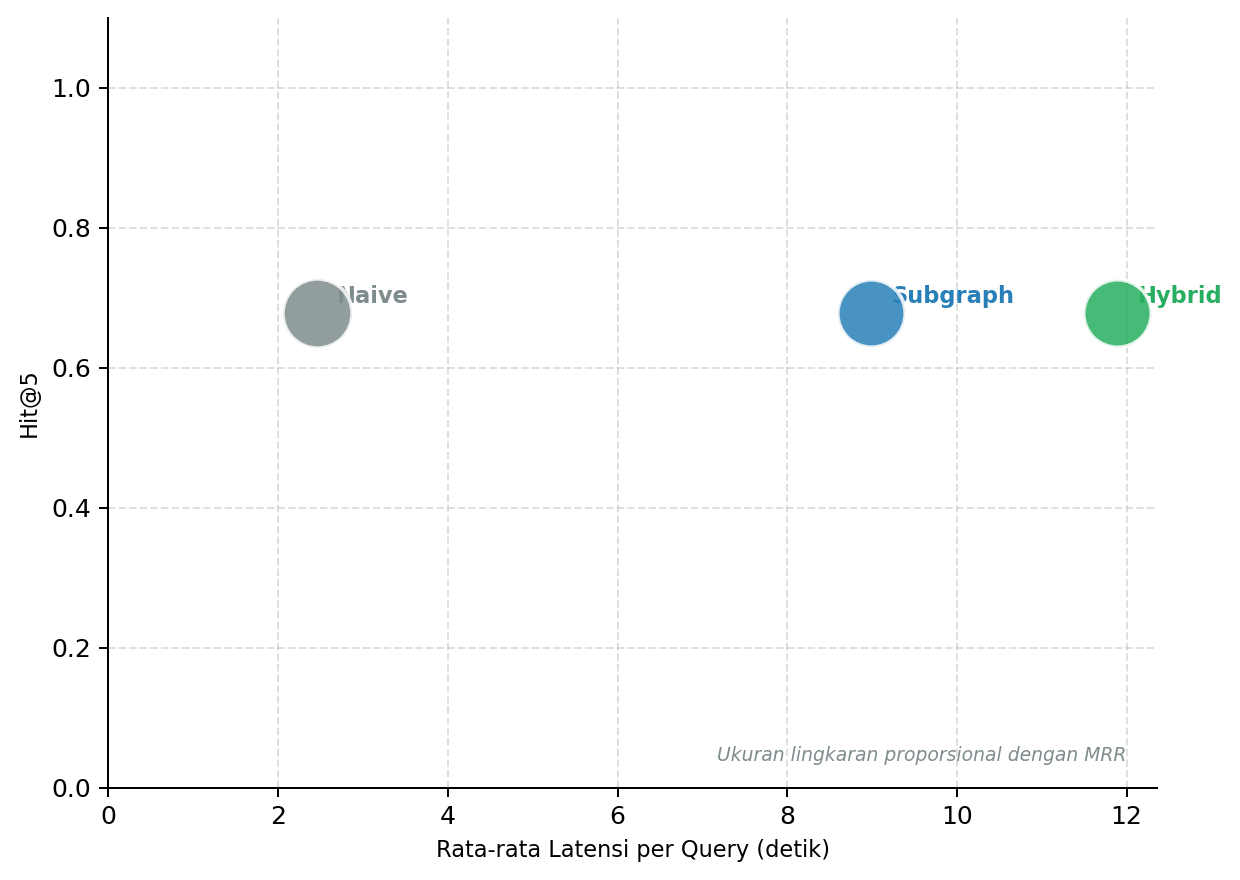
\includegraphics[width=0.82\linewidth]{Gambar/eval_layer3_latency_quality.png}
    \caption{Trade-off antara kualitas retrieval dan latensi.}
    \label{fig:eval-layer3-latency-quality}
\end{figure}

\begin{figure}[htbp]
    \centering
    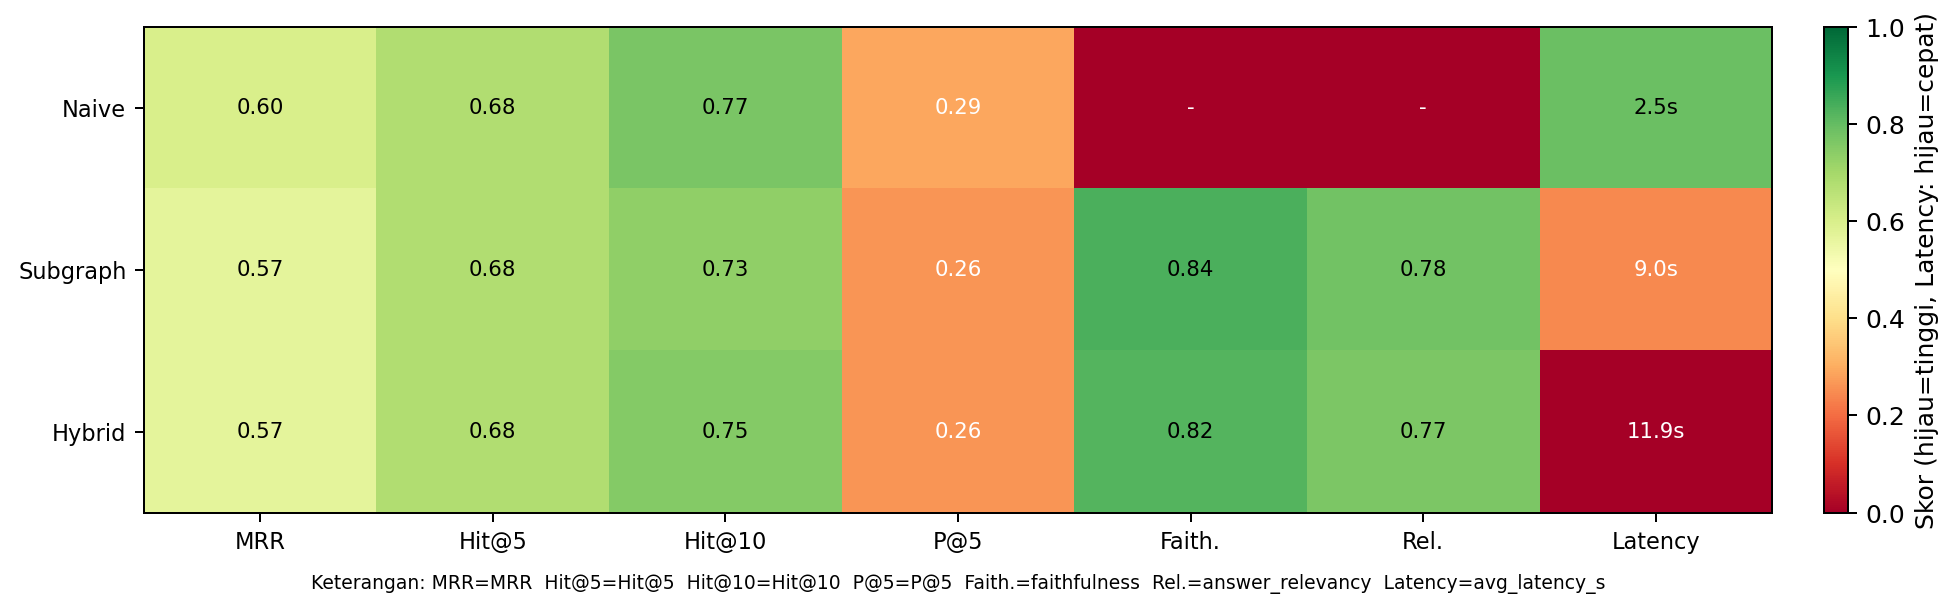
\includegraphics[width=0.86\linewidth]{Gambar/eval_layer3_scorecard.png}
    \caption{Scorecard perbandingan mode retrieval.}
    \label{fig:eval-layer3-scorecard}
\end{figure}

\begin{figure}[htbp]
    \centering
    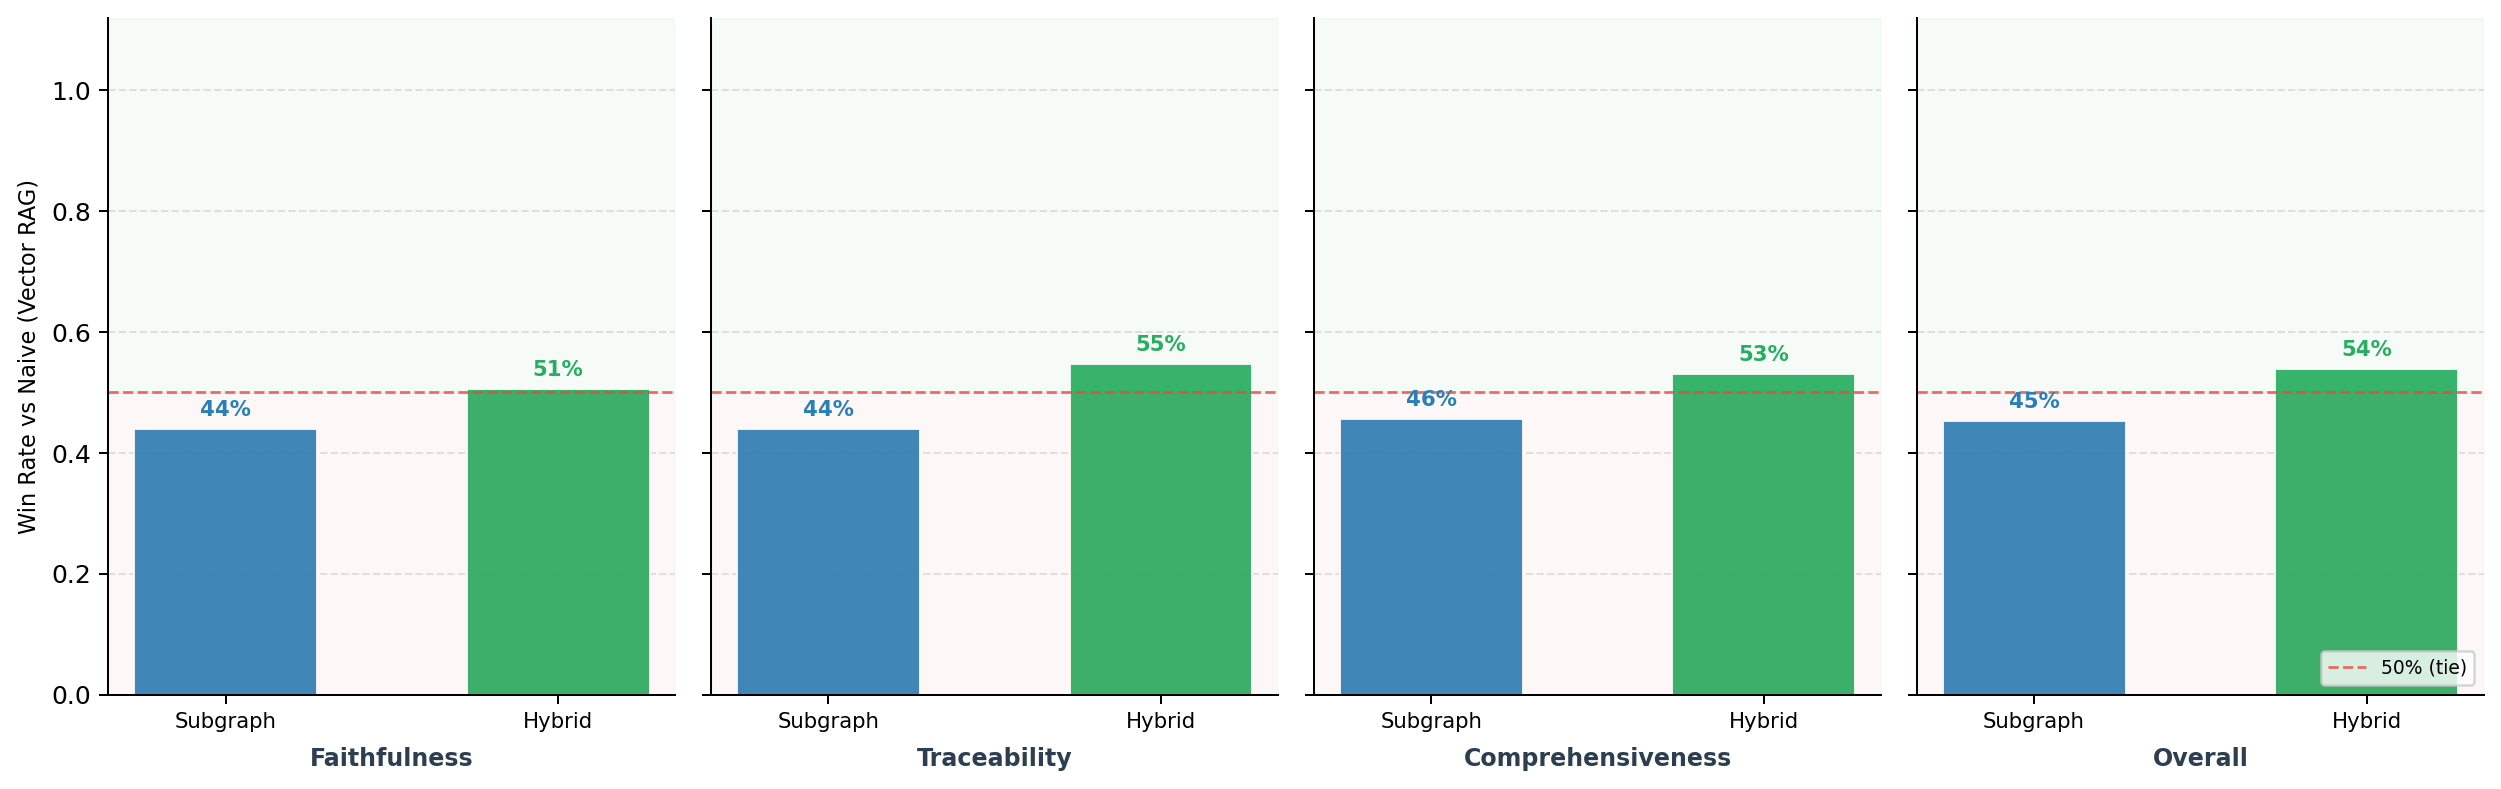
\includegraphics[width=0.82\linewidth]{Gambar/eval_layer4_winrate.png}
    \caption{Win rate LLM judge terhadap baseline Vector RAG.}
    \label{fig:eval-layer4-winrate}
\end{figure}

\begin{figure}[htbp]
    \centering
    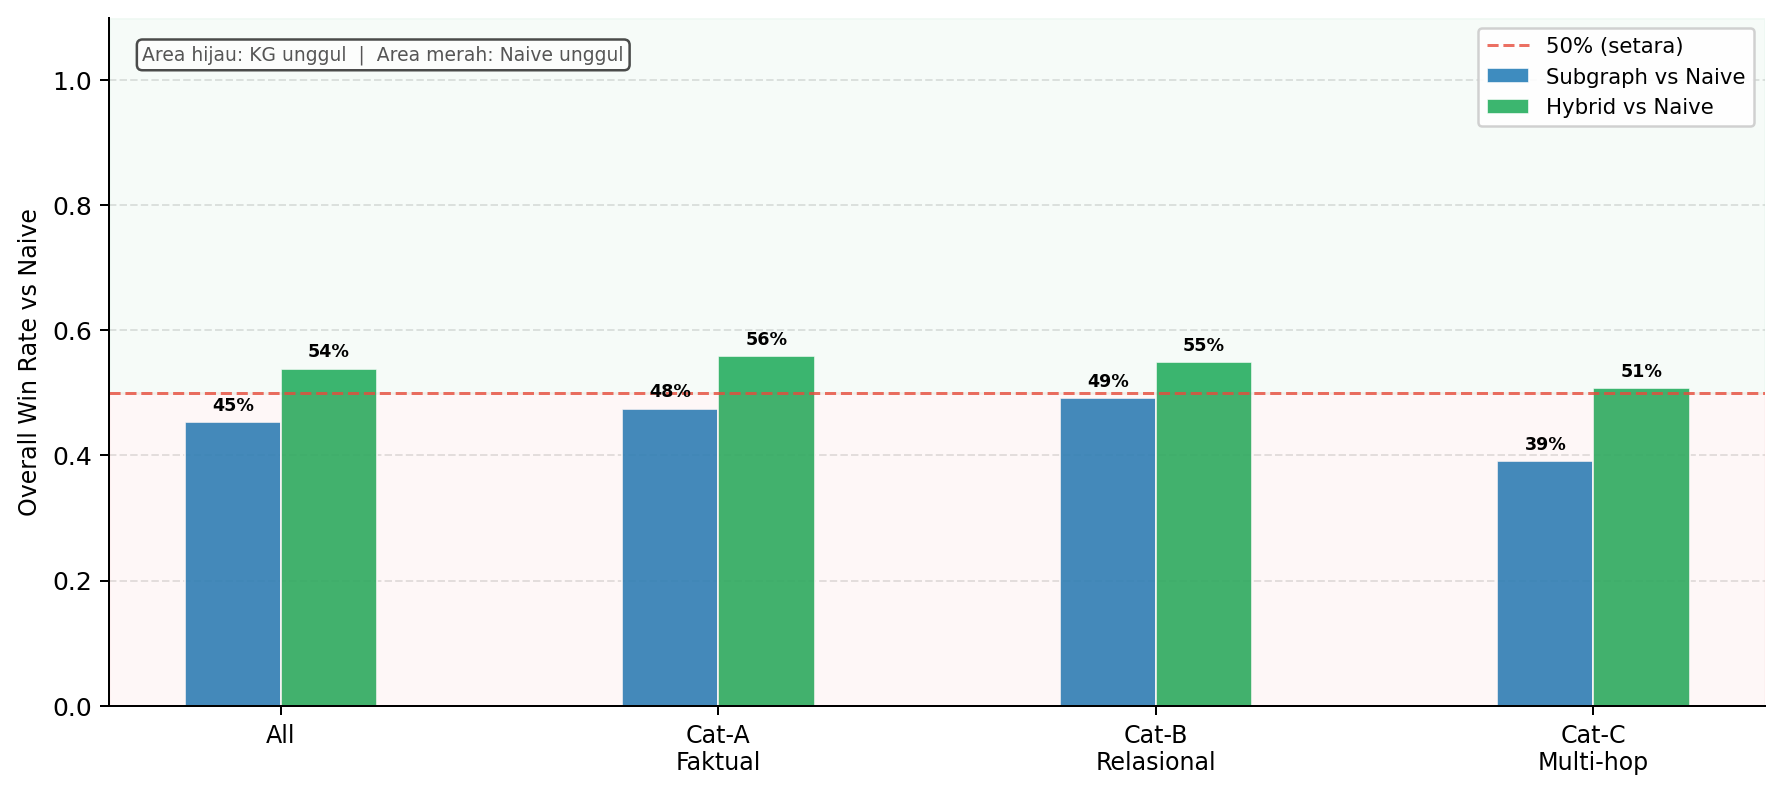
\includegraphics[width=0.82\linewidth]{Gambar/eval_layer4_category.png}
    \caption{Win rate LLM judge berdasarkan kategori pertanyaan.}
    \label{fig:eval-layer4-category}
\end{figure}

\begin{figure}[htbp]
    \centering
    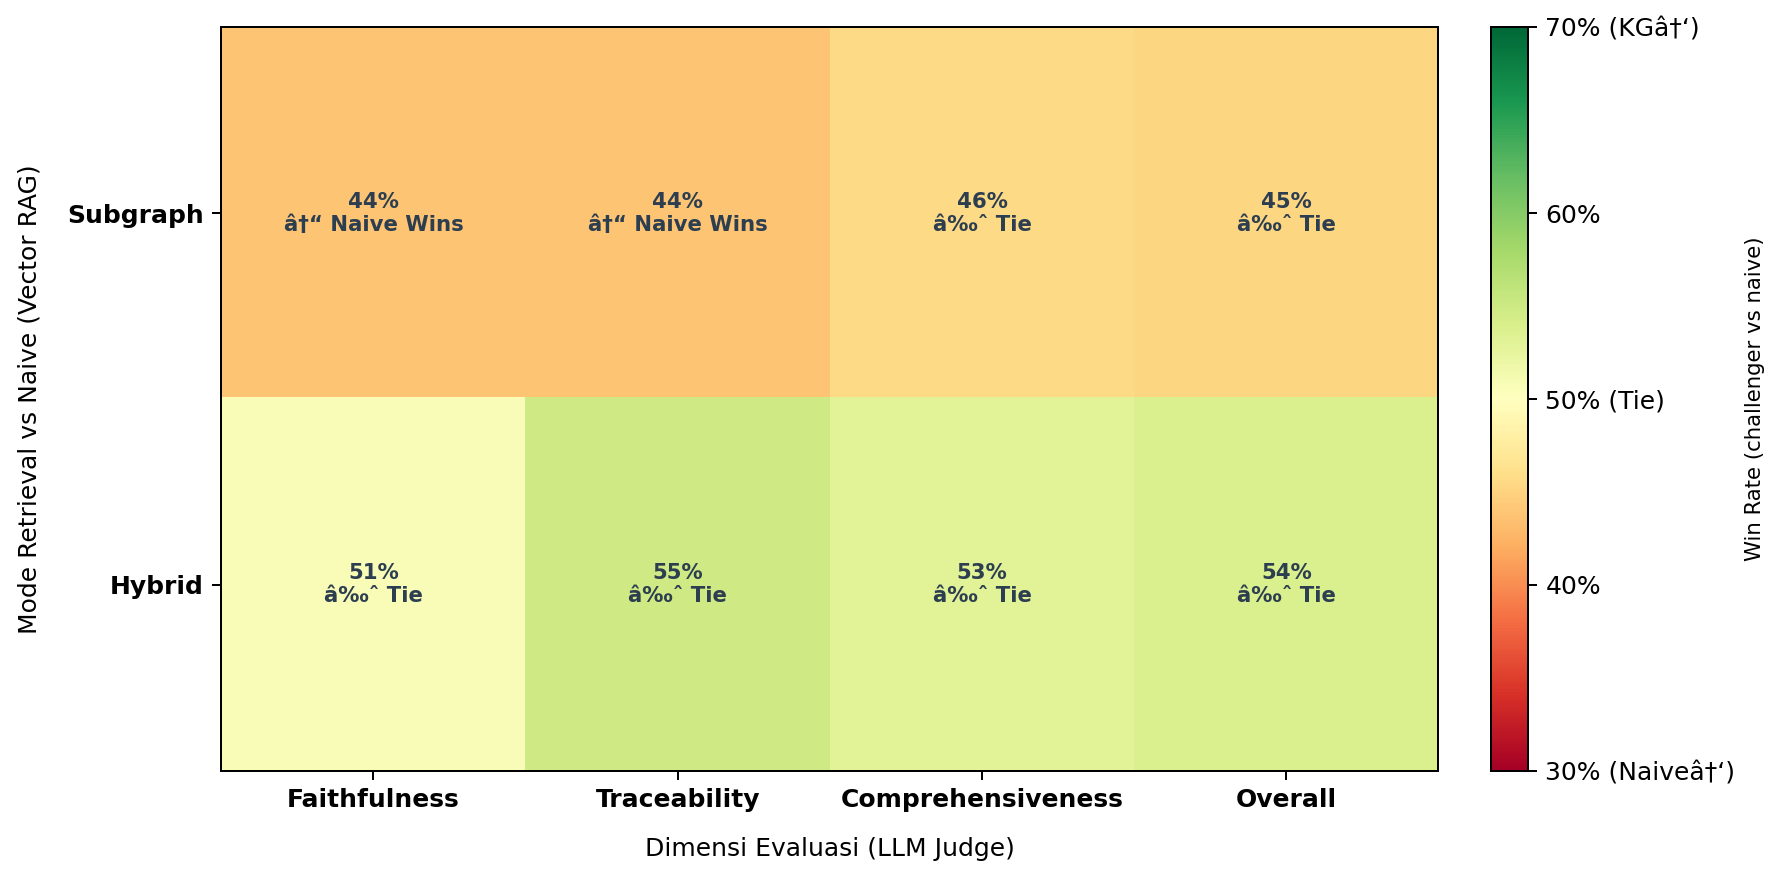
\includegraphics[width=0.90\linewidth]{Gambar/eval_layer4_heatmap.png}
    \caption{Heatmap hasil pairwise LLM judge per kasus evaluasi.}
    \label{fig:eval-layer4-heatmap}
\end{figure}

\begin{figure}[htbp]
    \centering
    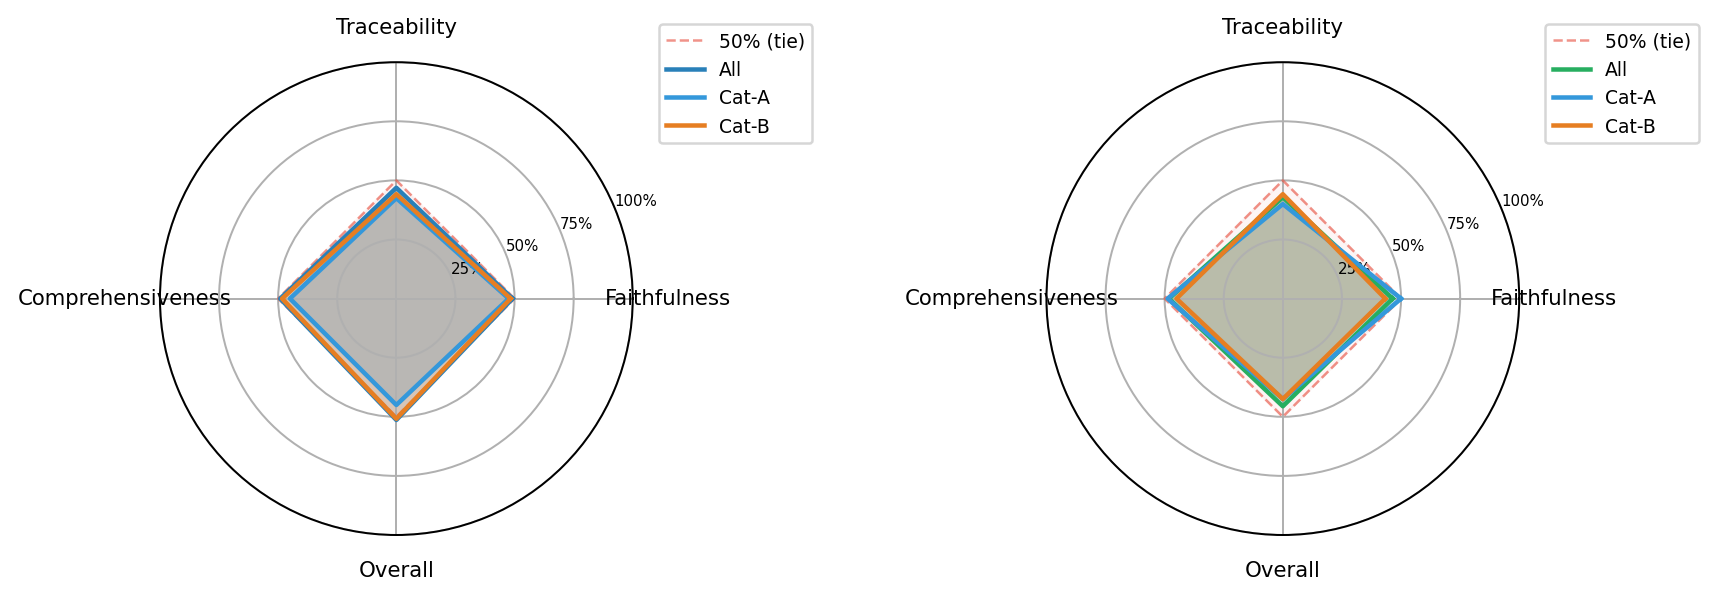
\includegraphics[width=0.76\linewidth]{Gambar/eval_layer4_radar.png}
    \caption{Perbandingan dimensi jawaban menurut LLM judge.}
    \label{fig:eval-layer4-radar}
\end{figure}
